\documentclass[10pt,reqno]{amsart}
\usepackage{amsmath}
\usepackage{amsthm}
\usepackage{amssymb}
\usepackage{graphicx}
\usepackage{mathrsfs}
\usepackage{color}
\usepackage{stmaryrd}
\usepackage{hyperref}
\usepackage{eucal}
\usepackage{fullpage}
\usepackage{algorithm}
\usepackage{algpseudocode}
\usepackage{tikz}
\usetikzlibrary{matrix,arrows}
\tikzset{node distance=2cm, auto}
\usepackage{outlines}
%%%%%%%%%%%%%%%%%%%%%%%%%%%%%%%%%%%%%%%%%%%%%%%%%%%%%%%%%%%%%%%%%%%%%%

\begin{document}

\noindent \textit{Math 363: Theory of Algorithms}

\noindent \textit{Instructor: Sreekar M.~Shastry}

\noindent \textit{Solutions to the Midterm Examination}

\noindent \textit{2012-03-02-Fri, 1530-1700}

\medskip

\begin{itemize}
    \item There are 6 problems. Each problem is worth 5 points. The
        maximum score is 30 points.
    % \item Clearly state the results which you invoke.
\end{itemize}

\medskip

\begin{outline}[enumerate]
\1 Let us recall the following definitions.

A \emph{queue} is a set from which we extract elements in first-in-first-out
(FIFO) order: we select elements in the same order in which they were added.
The procedure that adds an element is \texttt{Enqueue(Q,x)} and the procedure
that removes an element is \texttt{Dequeue(Q)}.

A \emph{stack} is a set from which we extract elements in last-in-first-out
(LIFO) order: we select the most recently added element. The procedure that
adds an element is \texttt{Push(S,x)} and the procedure that removes an element
is \texttt{Pop(S)}.

A \emph{max-priority queue} is a data structure that maintains a set of
elements $P$, where each element $v\in P$ has an associated value
$\mathtt{Key}(v)$ that denotes the priority of the element $v$; higher keys
represent higher priorities. Priority queues support the following procedures:
\texttt{Insert(P,x)} adds the element $x$ to $P$, \texttt{Maximum(P)} returns
the element of $P$ with the largest key, \texttt{ExtractMax(P)} removes and
returns the element of $P$ with the largest key (it returns \(-\infty\) if $P$
is empty), \texttt{IncreaseKey(P,x,k)} increases the value of element $x$'s key
to the new value $k$, which is assumed to be at least as large as $x$'s current
key value. Likewise one can define a \emph{min-priority queue} with procedures
\texttt{Insert, Minimum, ExctractMin, DecreaseKey}.

\2 Show how to implement a queue with a priority queue.
\2 Show how to implement a stack with a priority queue.

(For both (a) and (b), you may choose which type of priority queue to use.)

\medskip
\noindent \emph{Solution.} (a) We implement a queue by means of a min-priority
queue $P$.  Namely, we define \texttt{Enqueue(Q,x)} := \texttt{Insert(P,x)} and
\texttt{Dequeue(Q)} := \texttt{ExctractMin(P)}. In greater detail, given the
$i$th element $x_i$, we insert it into the min-priority queue with key value
$i$: $$\mathtt{Key}(x_i) = i.$$ Then the first call to \texttt{Dequeue(Q)}
returns $x_1$, the second call returns $x_2$ and so on, which demonstrates the
required FIFO property.

\medskip
(b) We implement a stack by means of a max-priority queue $P$.  We define
\texttt{Push(S,x)} := \texttt{Insert(P,x)} and \texttt{Pop(Q)} :=
\texttt{ExctractMax(P)}. In detail, given the $i$th element $x_i$, we insert it
into the max-priority queue with key value $i$: $$\mathtt{Key}(x_i) = i.$$
Suppose that the stack has $N$ elements at the time we issue a call to pop.
Then the first call to \texttt{Pop(Q)} returns $x_N$; if no other elements have
been pushed onto the stack, the second call returns $x_{N-1}$ and so on. On the
other hand, if some new element has been pushed onto the stack after the first
call to \texttt{Pop}, the next call to \texttt{Pop} will return the most
recently pushed element. This demonstrates the required LIFO property.

\medskip
Let us remark on the following distinction between (a) and (b).

\medskip
In the case of the FIFO queue, we have the following invariant: at all times
the set of key values present in the min-priority queue will be a consective
block of integers of the form $k, k+1, k+2,\dots,k+m$ for some positive
integers $k$ and $m$.

\medskip
In the case of a LIFO stack, at all times we are only guaranteed that the set
of key values in the max-priority queue is a strictly increasing set of
integers $k, k+i_1, k+i_2, \dots k + i_m$.

%\medskip
\newpage{}
\1 We call a graph $G=(V,E)$ a \emph{near-tree} if it is connected and has at
most $n+8$ edges, where $n := |V|$. Give an algorithm with running time $O(n)$
that takes a near-tree with edge costs and returns a minimum spanning tree of
$G$. You may assume that all of the edge costs are distinct.

\medskip

\noindent \emph{Solution.} The crucial subroutine is the following procedure
\textsc{DetectCycleByDepthFirstTraveral} which we will call simply $F$. It is a
modification of the depth first traversal algorithm. We maintain and update an
associative array $P$ which contains the partial DFS tree. (We remark that even
though $G$ is an undirected graph, once we specify a root vertex, the DFS tree
is a directed graph.) Thus $P[t] = s$ means that node $t$ has node $s$ as
parent on the DFS tree.

$F$ takes as input a graph $G$, a node $s$, and the node which is the parent of
$s$ in the depth first tree $P$. Note that $P$ is constructed by $F$ and grows
with each subsequent call to $F$.

$F$ returns the first nontrivial, non-tree edge $(u,v)$, else it returns NIL to
indicate that the graph $G$ is already a tree. By nontrivial non-tree edge, we
mean an edge that completes a nontrivial cycle in the undirected graph $G$; a
trivial cycle in an undirected graph is one of the form $s\rightarrow t
\rightarrow s$.

\medskip
\begin{algorithmic}[1]
    \State Let $P$ be a global variable, the associative array representing the DFS tree
    \State $s$ is the root node if and only if $P[s] = \mathtt{NIL}$
    %\State If $s_0$ is the root, $P[s_0] = \mathtt{NIL}$
    \Procedure{F}{$G, s$}
    \State Mark $s$ as explored
    \For{each edge $(s,t)$ incident to $s$}
    \If{$t$ is marked explored and $t\neq P[s]$}
    \State return $(s,t)$ \emph{// this edge completes a nontrivial cycle in $G$}
    \EndIf
    \If{$t$ is not marked explored}
    \State Let $P[t] := s$
    \State F$(G,t,P[t])$
    \EndIf
    \EndFor
    \State return \texttt{NIL}
    \EndProcedure
\end{algorithmic}
\medskip

Now, with the above subroutine in hand, we may describe the idea of the
algorithm to find an MST in a near-tree. We use $F$ to search for a cycle. If
there is no cycle, then the graph is a tree and we are done. Otherwise, we
delete the heaviest edge from the cycle. We do this 9 times.

\medskip
\begin{algorithmic}[1]
    \Procedure{NearTreeMST}{$G$}
    \State Choose an initial node $s$
    \For{$i =1,2,\dots, 9$}
    \State Let $(u,v) = F(G,s)$
    \If{$(u,v)=\mathtt{NIL}$}
    \State return \emph{// $G$ is already a tree}
    \EndIf
    \State Let $w = $ \textsc{LeastCommonAncestor}($u,v$)
    \State Let $e_1$ be the heaviest edge on the path from $u$ to $w$
    \State Let $e_2$ be the heaviest edge on the path from $v$ to $w$
    \State Delete from $G$ the heaviest of $e_1$, $e_2$, $(u,v)$ \emph{// to use the Cycle Property of MSTs}
    \EndFor
    \EndProcedure
\end{algorithmic}
\medskip

To analyze the complexity, write $n := |V|, m := |E|$, so that we have $n-1 \le
m \le n+8$ by connectedness and the near-tree property. The running time of $F$
is bounded by that of DFS which is $O(n+m) = O(n)$ on a near-tree.
\textsc{LeastCommonAncestor} takes $O(n)$ time (see page 96 of KT). Finding the
heaviest edge on a path takes $O(n)$ time, thus each of lines 9 and 10 takes
$O(n)$. The total running time of this algorithm is thus $O(9n) = O(n)$, as
required.

\medskip
% \1 Describe an algorithm that, given a set \(\{x_1,\dots,x_n\}\) of points on
% the real line, determines the smallest set of unit-length closed intervals
% that contains all of the given points. Show that your algorithm is correct.

\1 Dr.~Foo drives his car from Pune to Goa. When full, his car's gas tank holds
enough fuel to enable him to drive for $n$ kilometers. His gps navigation
system tells him in advance the distances between the gas stations on his
route. The doctor wishes to make as few gas stops as possible along the way.
Give an efficient algorithm by which Dr.~Foo may determine at which gas
stations to stop so as to achieve his goal of minimizing the total number of
gas stops. Prove that your algorithm is correct and determine its running time.

\medskip
\noindent \emph{Solution.} The optimal strategy goes as follows. Starting with
a full tank of gas, Foo should go to the farthest gas station at position $P_1$
from Goa which is at most $n$ miles from Pune. Starting from that point, he
should go to the farthest gas station $P_2$ which is within $n$ miles of
position $P_1$. And so on.

Put differently, at each gas station, Foo should ask whether he can make it to
the next gas station without stopping at this one. If he can, skip this one.
This description shows that the algorithm is $O(m)$, where $m$ is the total
number os stations.

(i) Now, consider an optimal solution with $s$ stations which stops first at
the $k$th station. Then we claim that the rest of the optimal solution must be
an optimal solution to the subproblem of the remaining $m-k$ stations. If this
were not the case, we could find a solution to the problem on $m-k$ stations
which stopped at $< s-1$ stations and we could use this to construct an optimal
solution on $m$ stations with $< s$ stops, contradicting our supposition.

(ii) Moreover, any optimal solution must choose as the first station the
farthest station (the $k$th station, say) which is within $n$ miles of Pune.
For if not and we had chosen the $j$th station with $j<k$, then upon leaving
the $j$th station we could get no further than if we stopped at the $k$th
station. Thus stopping at station $j < k$ results in a solution which can do no
better than stopping at the $k$th station.

Taken together, (i) and (ii) prove that our algorithm is correct.

\medskip

\1 We are given two sets $A$ and $B,$ each consisting of $n$ positive integers.
You may reorder the sets in any manner you choose. After reordering, write
$a_i$ for the $i$th element of $A$ and $b_i$ for the $i$th element of $B$. The
payoff obtained from the chosen orderings is \[\prod_{i=1}^n a_i^{b_i}.\]
\2 Give an algorithm which maximizes the payoff.
\2 Prove the correctness of your answer to part (a) and determine its running
time.

\medskip
\noindent \emph{Solution.} Sort $A$ and $B$ into decreasing order.
\medskip

To prove that this yields the optimal solution, we argue as follows. Let $i <
j$ and consider $a_i^{b_i}$ and $a_j^{b_j}$. Let us show that
$a_i^{b_i}a_j^{b_j} \ge a_i^{b_j}a_j^{b_i}$. Since we have sorted $A$ and $B$
into decreasing order, $a_i \ge a_j$ and $b_i \ge b_j$. Since $a_i, a_j > 0$
and $b_i-b_j \ge 0$, we have $a_i^{b_i-b_j} \ge a_j^{b_i-b_j}$. Multiplying
both sides by $a_i^{b_j}$ yields $a_i^{b_i}a_j^{b_j} \ge a_i^{b_j}a_j^{b_i}$.

\medskip
Since multiplication of real numbers is commutative, sorting $A$ and $B$ into
increasing order also would have worked.  What the above argument actually
demonstrated was that we must choose compatible orderings on $A$ and $B$ in the
sense that for both sets, for all $i$, the $i$th element must be the $i$th
element from the top or that for all $i$, the $i$th element is the $i$th
element from the bottom.

\medskip
The running time is the running time the sorting algorithms we know
(e.g.~mergesort): $O(n\log n)$.

\medskip
\1 This problem is about Huffman coding.
\2 Explain the relationship between prefix codes and binary trees.
\2 Show that the binary tree corresponding to the optimal prefix code must be full.

\medskip
\noindent \emph{Solution.} (a) This is in section 4.8 of KT.

(b) This is proposition 4.28 on page 168 of KT.

\medskip
\1 This problem is about Dijkstra's algorithm for computing the \emph{length}
of the shortest path from a given root to any other vertex.
\2 State Dijkstra's algorithm.
\2 Give a simple example of a directed graph with some edges having negative
length for which Dijkstra's algorithm produces an incorrect answer.

\medskip
\noindent \emph{Solution.} (a) This is in KT on page 138.

(b) In the following figure, we start from s. Dijkstra's algorithm tells us
that the distance from s to y is 1, but going the long way around shows that
the distance is 0.

\begin{center}
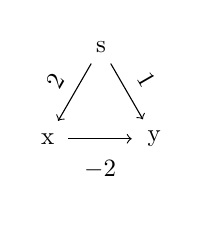
\begin{tikzpicture}[scale=.9, transform shape]
%\tikzstyle{every node} = [circle, fill=gray!30]
\tikzstyle{every node} = [circle]
\node (x) at (0, 0) {x};
\node (y) at +(0: 1.5) {y};
\node (s) at +(60: 1.5) {s};
%\foreach \from/\to in {s/x, s/y, x/y}
%\draw [->] (\from) -- (\to);
\draw [->] (s) -- (x) node[pos=0.5, sloped, above] {$2$};
\draw [->] (s) -- (y) node[pos=0.5, sloped, above] {$1$};
\draw [->] (x) -- (y) node[pos=0.5, sloped, below] {$-2$};
\end{tikzpicture}
\end{center}

\end{outline}
\end{document}
